    A continuación se muestran las figuras obtenidas con el procedimiento obtenido anteriormente.

    \begin{figure}[h!]
        \centering
        \begin{minipage}[t]{0.48\textwidth}
            \centering
            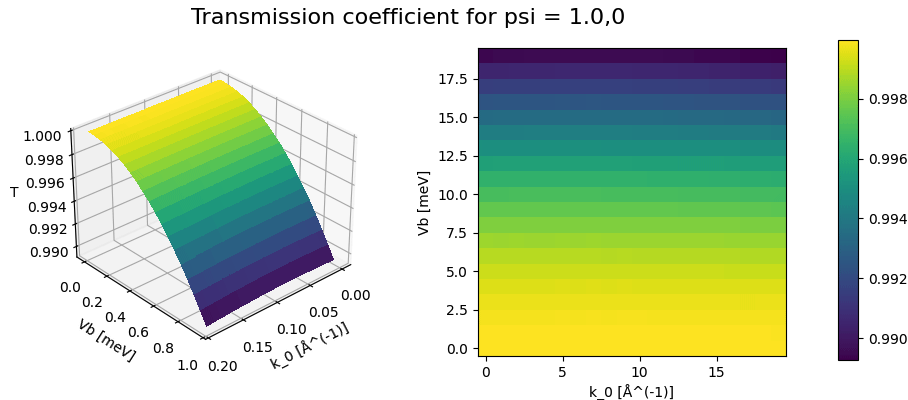
\includegraphics[width=\textwidth]{../assets/images/No-Rashba/TCoefficient(1.0,0)xalpha=0beta=0}
            \caption{figure}{
Transmission coefficient (T) in pristine graphene with initial pseudospinor configuration $\xi = (1, 0)$, plotted against potential barrier height (Vb, in meV) and initial wave vector ($k_0$, in $\angstrom^{-1}$). The 3D plot and 2D heatmap show that transmission is largely independent of the initial wave vector but decreases noticeably as the barrier height increases, ranging from $1$ to approximately $0.990$.
}
            \label{fig:noRashba}
        \end{minipage}
        \hfill
        \begin{minipage}[t]{0.48\textwidth}
            \centering
            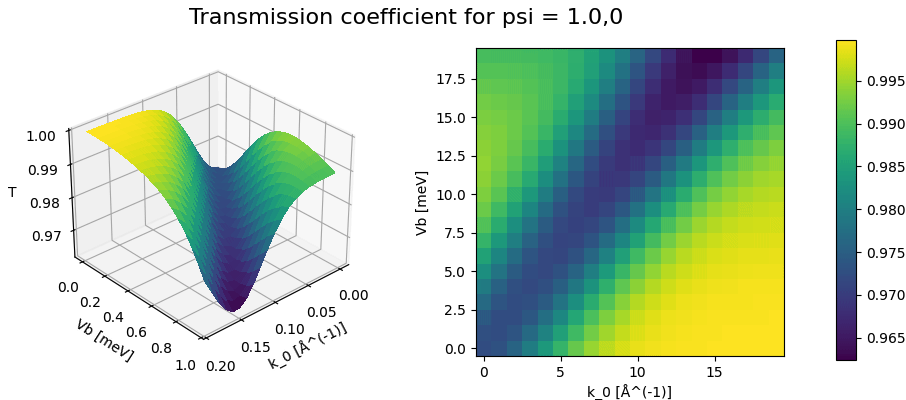
\includegraphics[width=\textwidth]{../assets/images/Rashba/TCoefficient(1.0,0)xalpha=0.2beta=-0.2}
            \caption{figure}{
Coeficiente de transmisión ($T$) en función de la altura de la barrera de potencial ($Vb$) y el número de onda inicial ($k_0$) con una configuración inicial de pseudoespinor $\xi = (1, 0)$. La superficie 3D y el mapa de color 2D muestran una dependencia no monotónica de $T$ con respecto a $Vb$ y $k_0$, destacando la influencia del acoplamiento espín-órbita en la transmisión a través de la barrera.
}
            \label{fig:rashba}
        \end{minipage}
    \end{figure}

    En las imágenes podemos notar ciertos aspectos interesantes, empezando con la fig.\ref{fig:noRashba}.
    La imagen presenta dos gráficos que ilustran el coeficiente de transmisión ($T$) en función de $Vb$ (en meV) y $k_0$ (en $\angstrom^{-1}$) para un valor fijo de $\xi = (1, 0)$.
    El gráfico de la izquierda es una visualización tridimensional donde $T$ está en el eje $z$, $Vb$ en el eje $x$ y $k_0$ en el eje $y$, con una escala de colores que varía desde morado oscuro (menor $T$) hasta amarillo brillante (mayor $T$). El gráfico de la derecha es un mapa de calor bidimensional que ofrece una vista superior, con el eje $x$ representando $k_0$ y el eje $y$ representando $Vb$, usando el mismo mapa de colores que el gráfico 3D\@.
    Ambos gráficos muestran que el coeficiente de transmisión generalmente se mantiene muy cerca de 1, indicando una alta transmisión.
    Conforme aumenta $Vb$, $T$ tiende a disminuir, mientras que la dependencia respecto a $k_0$ es mínima.
    En general, los gráficos demuestran cómo cambia $T$ con variaciones en $Vb$ y $k_0$, destacando una leve disminución de $T$ al aumentar $Vb$ y un cambio insignificante respecto a $k_0$.

    Este resultado muestra una contradicción con lo que ya se especifíca en la literatura, en el grafeno se esperaría observar una transmisión total debido a las mismas propiedades del material\cite{horsell2008, Young2009}.

    The previously described behavior might be the result of one or both of the following aspects:

    \begin{itemize}
        \item Wave Packet Characteristics:
        Not a single momentum eigenstate.
        Debido a que estamos ocupando paquetes de onda en la simulación, un detalle importante que surge es que existe la presencia de múltiples componentes de momentum y eso implica que algunos de ellos pueden causar interferencia con otros; causando un coeficiente de transmisión que difiere del de un solo autoestado\cite{Staelens2021}.
        Además, en nuestra simulación se está tomando en cuenta el tiempo.
        Parte de la investigación a futuro es comprobar si el tiempo de fase o de tunelaje están directamente relacionados a la variación del coeficiente de transmisión observada en este trabajo.
        \item Quantum interference effects\cite{MolgadoMex2018}.
        Dependiendo del ancho del paquete y su amplitud, este se puede dispersar con el tiempo y esto puede causar interferencia consigo mismo.
        Conforme diferentes partes del GWP encuentran la barrera de potencial, estos pueden estar interfiriendo, causando fluctuaciones en el coeficiente de transmisión.
    \end{itemize}

    Por otro lado, tenemos la transmisión bajo presencia de SOIR (Fig.\ref{fig:rashba}).

Se observa una correlación entre las variables: generalmente, a mayor altura de la barrera de potencial ($Vb$) y mayor número de onda inicial ($k_0$), se espera una menor transmisión.
Sin embargo, la interacción espín-órbita introduce un comportamiento más complejo.
A medida que $k_0$ aumenta y $Vb$ disminuye, la transmisión se acerca a 1, indicando una mayor probabilidad de tunelamiento cuántico debido a la SOIR\@.

Aunque la variación en el coeficiente de transmisión es pequeña (del orden de $10^{-2}$), es significativa y atribuible a la interacción SOIR. Los electrones, con sus diferentes componentes de pseudoespín, interactúan, y esta interacción se ve afectada por el número de onda inicial del paquete de ondas gaussiano (GWP), como se observó en estudios previos\cite{Serna2019}.
Por lo tanto, la SOIR modula la interacción, lo que a su vez causa las fluctuaciones observadas en el coeficiente de transmisión.





% Conclusions